\section{Discussion and Future Work}
\label{sec:discuss}

We next discuss issues in our approach and describe how we address
these issues in our future work.

\textbf{Aligning client code.} Table~\ref{table:analyzingclient}
shows that our approach could not align client code in a few cases.
The primary reason is that the functionality associated with a class
or a method in one language version is split among multiple classes
or methods in the other language version. To address this issue, we
plan to align classes and methods of client code based on their
functionalities through developing or adapting dynamic approaches~\cite{jiang2009automatic} in future work.

\begin{figure}[t]
\centering
\includegraphics[scale=1,clip]{figure/n2n.eps}\vspace*{-3ex}
 \caption{Merging technique}\vspace*{-3.5ex}
 \label{fig:n2n}
\end{figure}

\textbf{Mining richer API mapping.} Table~\ref{table:compare} shows
that our approach does not achieve very high recall for J2SE. Although we
use 10 large projects as subjects, these projects still do not
provide sufficient code examples for mining mapping relations of all
APIs in J2SE. Our previous
work~\cite{thummalapenta07parseweb,thummalapentaase08spotweb} show
that it is feasible to use large-scale repositories available on the
web as subjects with the help of code search engines such as Google
code search\footnote{\url{http://www.google.com/codesearch}}. In
future work, we plan to leverage these code search engines to mine
richer API mapping.

%(@Hao: This ranking mined mapping relations sound very trivial. Can we ignore this?)
%\textbf{Ranking mined mapping relations.} When comparing with the
%built mapping files of Java2CSharp, we choose mined mapping
%relations of APIs with the highest supports as generated mapping
%files. However, in some cases, the API mapping with the highest
%support is not necessarily the best choice. For example,
%\CodeIn{java.util. ArrayList} is mapped to
%\CodeIn{System.Collections.ArrayList} based on support values. The
%Java class supports generic programming, whereas the C\# class does
%not. Consequently, the Java class seems to be better mapped to
%\CodeIn{System.Collections.Generic.List} as this C\# class also
%supports generic programming. We plan to develop ranking techniques
%to address this issue in future work.

\textbf{Mining many-to-many mapping relations of API methods.} Among
our mined mapping relations of API methods, many relations are
one-to-one relations. The reason is that our Algorithm 2 uses only
forward analysis for merging API methods. We explain this issue
using an illustrative example shown in Figure~\ref{fig:n2n}. After
merging API methods \CodeIn{method1} and \CodeIn{method2}, if our
algorithm is still not able to map the merged API methods with an API
method in the other language, our algorithm attempts to merge
\CodeIn{method3} rather than \CodeIn{method4}, which could be a
possible candidate for mining the mapping relation. In future work,
we plan to incorporate backward analysis to enhance our existing
algorithm. We expect that our enhanced algorithm can mine more
many-to-many mapping relations.

\textbf{Migrating many-to-many mapping relations of API methods.}
A mined many-to-many mapping relation of API methods can have multiple outputs
and complex internal data processes. Although our ATGs
help identify all API methods, our implementation is not complete
for supporting automatic translation. For example, we need to manually add an
\emph{or} operator for the two outputs of the API mapping shown in
Figure~\ref{fig:example}. In future work, we plan to enhance our implementation to help
automate migration with many-to-many mapping relations.

\textbf{Migrating unmapped APIs.} Our approach mines API mapping of
methods along with the mappings of their inputs and outputs. These
mappings are useful for translating API methods of one language to
another. Sometimes, our approach may not be able to map inputs and
outputs of mapped API methods. If our approach is not able to map
outputs, our approach currently simply ignores those outputs that are not used
in the client code. However, since inputs cannot be ignored, the
translated code has compilation errors. In future work, we
plan to address this issue by analyzing how two versions of a
project deal with a similar unmapped API problem for some other code
examples.
